\documentclass{article}
\usepackage{graphicx}
%pages setting
\usepackage{geometry}
\geometry{a4paper, centering, scale = 0.8}

\title{COMSM0104-Web Technologies Report}
\author{Kehan Du, Shunyi Zhao}

\begin{document}

\maketitle

\section{Introduction}
Our team is comprised of Kehan Du (mz19460) and Shunyi Zhao (vt19049). The
aim of our project is constructing the PC end official website of Deep KW
Innovation Factory.

~\\
\noindent
Deep KW Innovation Factory is the academic workshop of interdisciplinary 
at Huazhong University of Science and Technology, China. Since the establishment 
of Deep KW Innovation Factory in 2017, it has always upheld and practiced 
the concepts and methods of interdisciplinary, and insisted on exploring 
the question of social sciences by using natural science methods.

~\\
\noindent
The central goal of this version is to construct of the official website 
framework and the dynamic realization of key pages and complete the initial 
launch of the official website. This version is just used to practice the skills
of web technologies, and will not be used commercially. We have got the
permission to do this website, and each work we cite will be quoted exactly in
the final submission.

\section{Page Design}
The home page of this project is shown below:
\\
\begin{figure}[h]
    \centering
    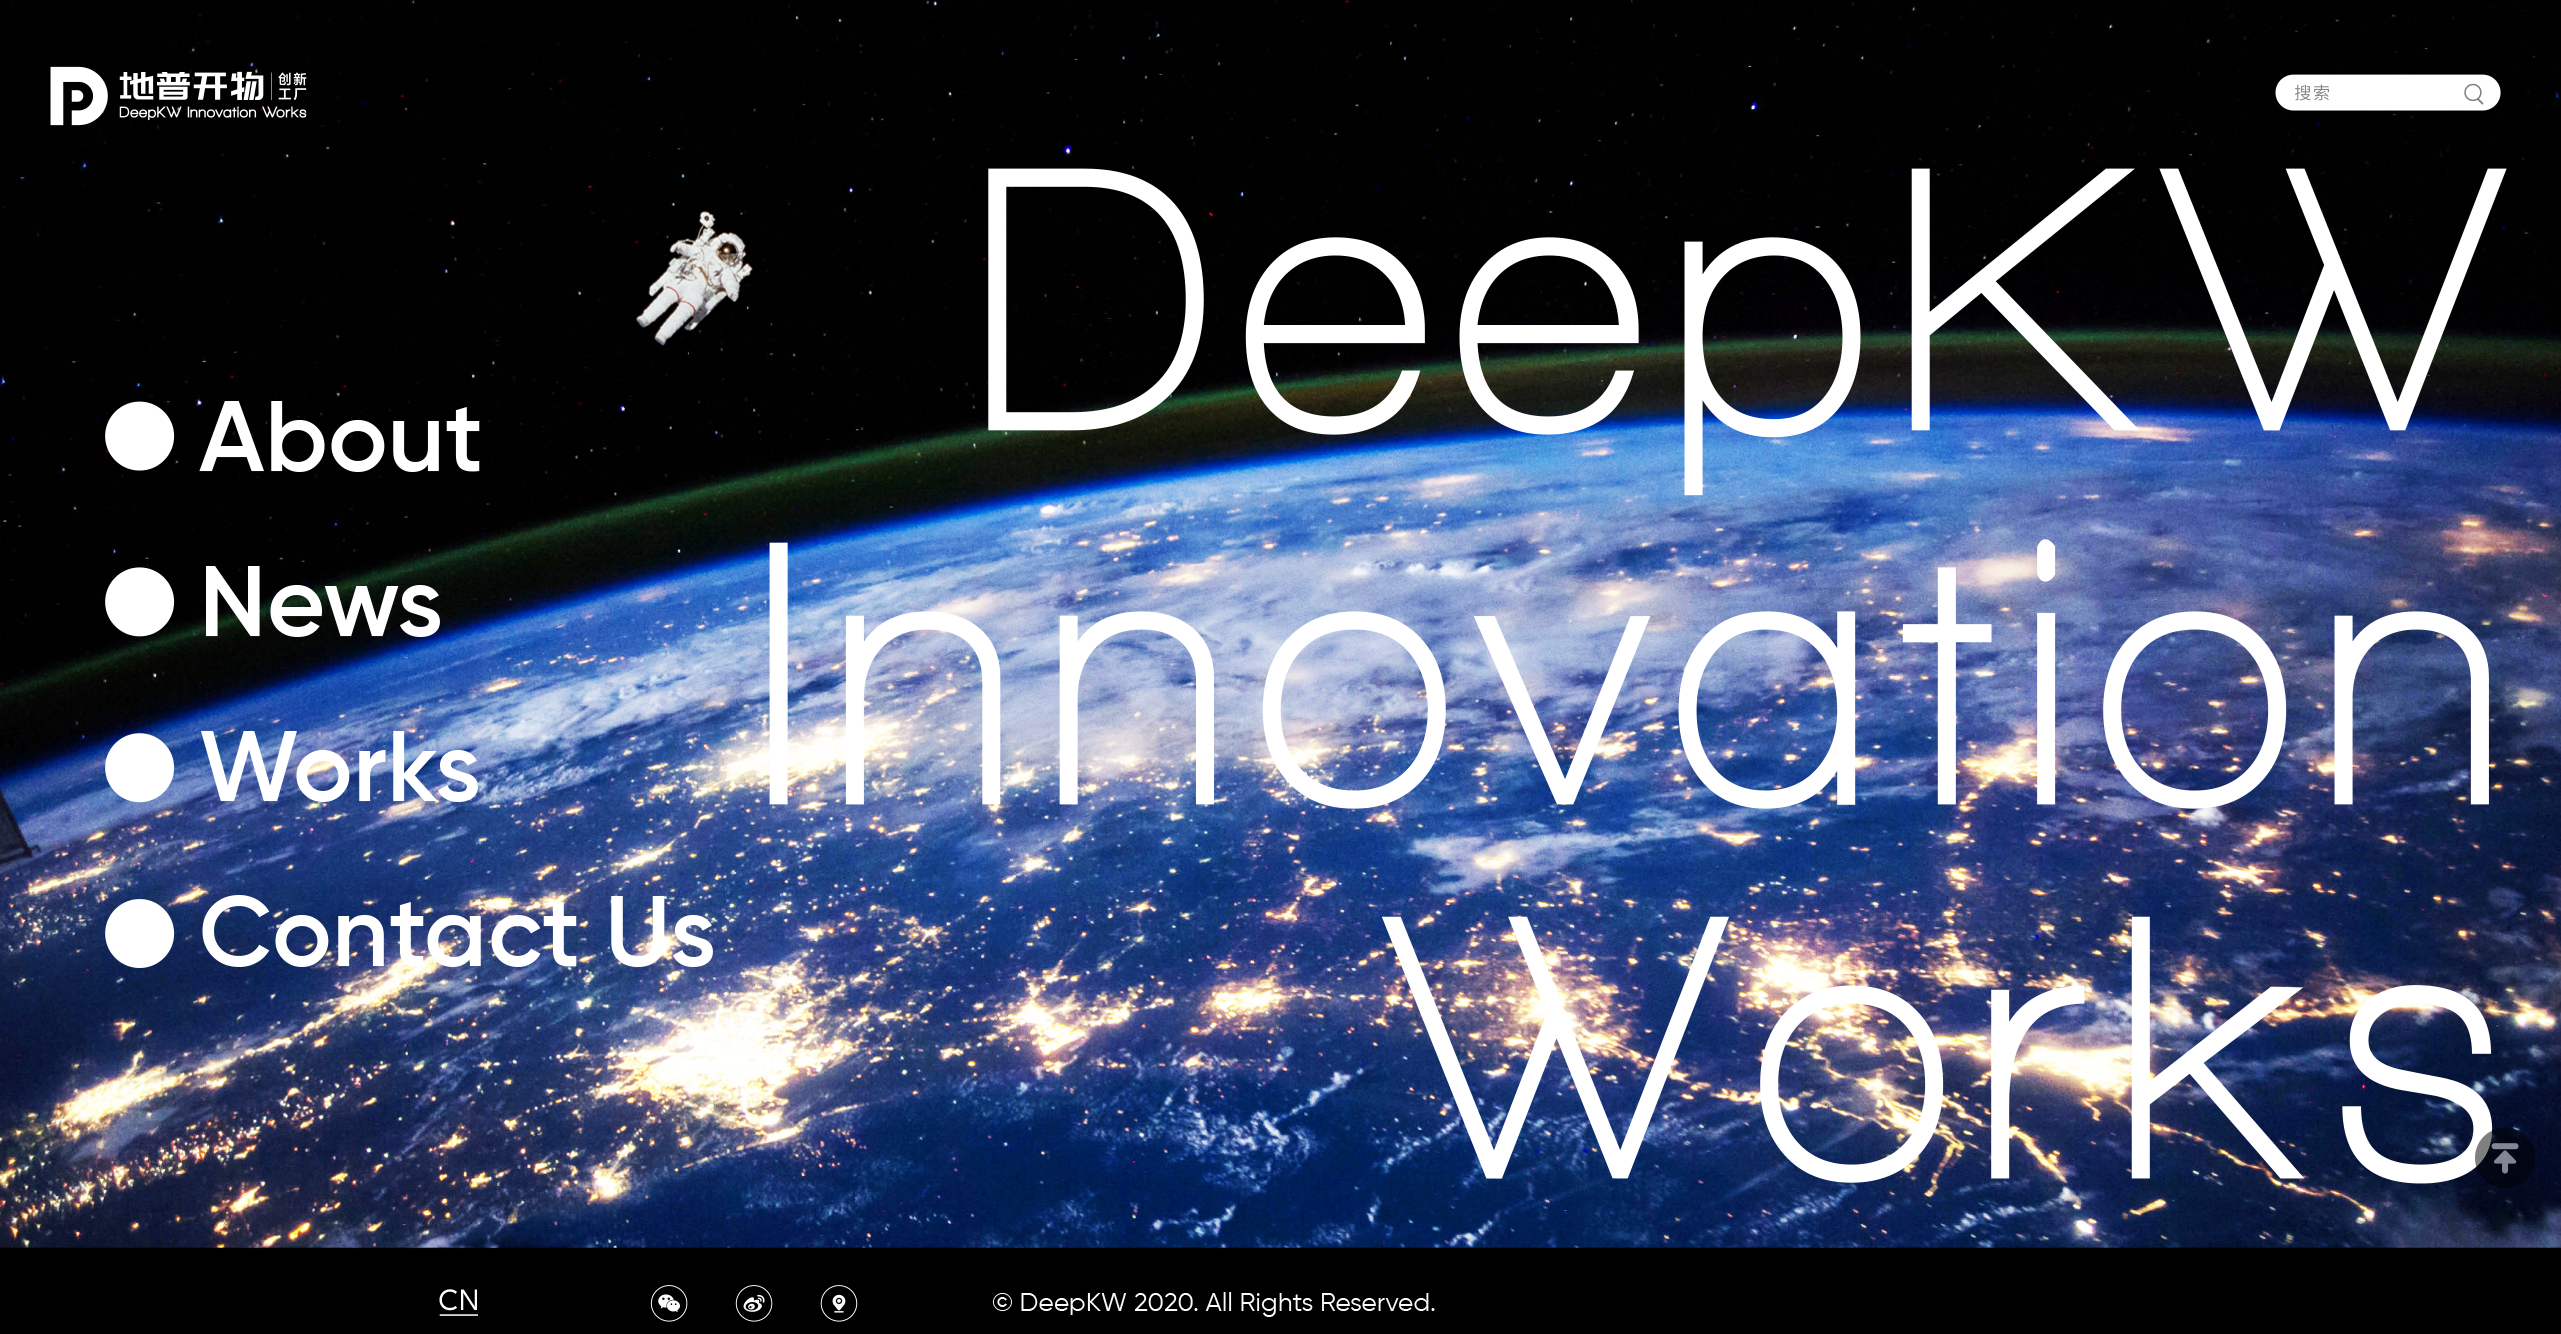
\includegraphics[height=4cm]{img/02.png}
    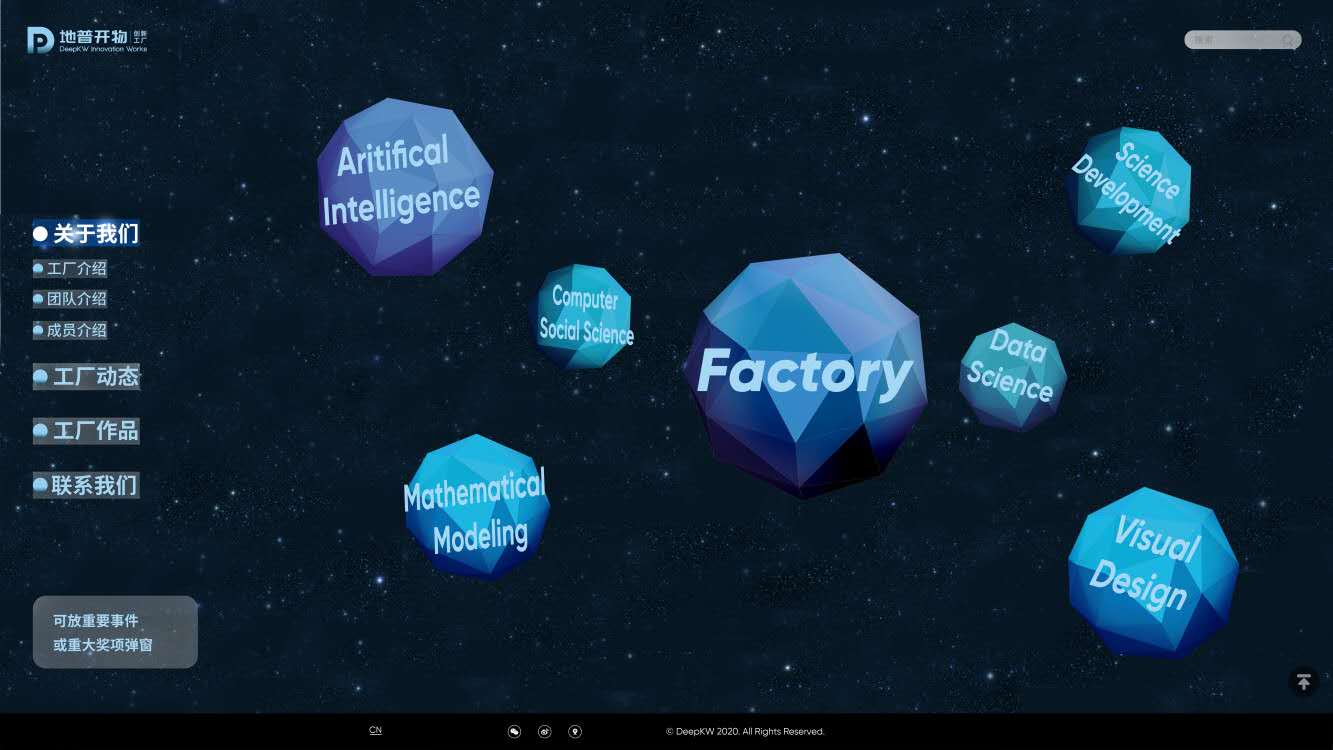
\includegraphics[height=4cm]{img/05.jpg}
    \caption{home page and about page}
    \label{fig: homepage}
\end{figure}
\\
\section{Technology Evaluation}
\subsection{Client Side}
We chose a popular javascript framework, Vue.js (version 2.6.11), to 
develop these pages.
Modularity and componentization are important features of Vue,  
allowing us to build complex applications with small, independent, 
and usually reusable components. And these components convenient 
for later maintenance and upgrade of the official website. 
We use node.js and npm manage the packages, and 
information about these packages are shown in package.json. Works are 
placed in folder named \textit{./src/components}. HTML are used as 
the template of every module, CSS statemens would control the layout 
and style of these modules.

~\\
\noindent
Adobe Photoshop and Illustrator (Authorized) are used to design the 
blueprint of the website, and some .png file are created by them. 
Some icons, such as the logo of group, are drawn by SVG.

\subsection{Sever Side}
Development of Sever is also in node.js.
Express and Sqlite are used to control Database. And the concept page shown
before homepage will be displayed by a dynamic page.


    
\end{document}
